\documentclass[11pt]{article}
\input{preamble.tex}
\input{preamble-cours.tex}

\solutionstrue

\begin{document}

\chapitre{7}{Invariants}

De nombreux problèmes d'olympiades décrivent une situation que l'on transforme
en répétant une même opération. On demande alors si un certain état peut être
atteint, si le processus doit s'arrêter, ou quelle sera sa configuration finale.

Essayer toutes les suites d'opérations est souvent impossible. L'idée consiste
plutôt à chercher une propriété qui ne change jamais au cours du processus :
un \textbf{invariant}.

\section{Exemple introductif : retourner des jetons}\label{sec:exemple-introductif}

On dispose de \(8\) jetons, tous placés face blanche visible.

À chaque opération, on doit retourner exactement deux jetons.

Peut-on obtenir une configuration contenant exactement un jeton noir ?

\begin{center}
\fitfig{%
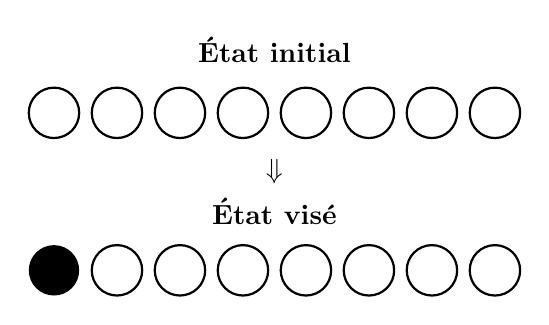
\begin{tikzpicture}[x=1cm,y=1cm,line width=0.8pt]
    \node at (3.5,2.8){\textbf{État initial}};
    \foreach \x in {0.7,1.5,2.3,3.1,3.9,4.7,5.5,6.3} \draw (\x,2) circle (0.32);
    \node at (3.5,1.25){\(\Downarrow\)};
    \node at (3.5,0.75){\textbf{État visé}};
    \fill (0.7,0) circle (0.32);
    \foreach \x in {1.5,2.3,3.1,3.9,4.7,5.5,6.3} \draw (\x,0) circle (0.32);
\end{tikzpicture}}
\end{center}

Notons \(N\) le nombre de jetons noirs.

Lorsqu'on retourne deux jetons, trois situations sont possibles :

\begin{itemize}
    \item deux jetons blancs deviennent noirs : \(N\) augmente de \(2\) ;
    \item un jeton blanc et un jeton noir sont retournés : \(N\) ne change pas ;
    \item deux jetons noirs deviennent blancs : \(N\) diminue de \(2\).
\end{itemize}

Ainsi, à chaque opération,

\[
N\longmapsto N+2,\qquad N,\qquad\text{ou}\qquad N-2.
\]

La parité de \(N\) ne change donc jamais.

Au départ,

\[
N=0,
\]

qui est pair. Après n'importe quel nombre d'opérations, \(N\) reste pair.

Or l'état demandé contient exactement un jeton noir, donc

\[
N=1,
\]

qui est impair.

L'état demandé est donc impossible à atteindre.

\[
\boxed{
\text{La parité du nombre de jetons noirs est un invariant.}
}
\]

\section{Le concept d'invariant}\label{sec:concept-invariant}

\subsection{Définition}\label{sec:definition-invariant}

\begin{definition}[Invariant]
Un \textbf{état} décrit complètement la situation à un instant donné.

Une \textbf{opération autorisée} transforme un état en un autre.

Une quantité \(I\) est appelée un \textbf{invariant} lorsqu'elle conserve
toujours la même valeur après chaque opération autorisée.

Autrement dit, si un état \(S\) est transformé en un état \(S'\), alors

\[
\boxed{I(S')=I(S).}
\]
\end{definition}

On peut représenter le principe ainsi :

\begin{center}
\fitfig{%
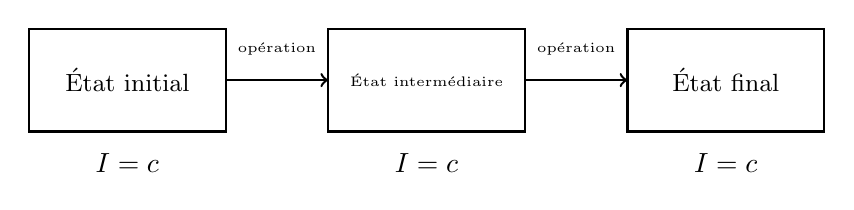
\begin{tikzpicture}[x=1cm,y=1cm,line width=0.9pt]
    \draw (0,0.5) rectangle (2.5,1.8);
    \draw (3.8,0.5) rectangle (6.3,1.8);
    \draw (7.6,0.5) rectangle (10.1,1.8);
    \node at (1.25,1.15){\small{État initial}};
    \node at (5.05,1.15){\tiny{État intermédiaire}};
    \node at (8.85,1.15){\small{État final}};
    \draw[->] (2.5,1.15)--(3.8,1.15);
    \draw[->] (6.3,1.15)--(7.6,1.15);
    \node at (3.15,1.55){\tiny{opération}};
    \node at (6.95,1.55){\tiny{opération}};
    \node at (1.25,0.1){\(I=c\)};
    \node at (5.05,0.1){\(I=c\)};
    \node at (8.85,0.1){\(I=c\)};
\end{tikzpicture}}
\end{center}

\begin{proposition}
Si l'état initial et l'état visé n'ont pas la même valeur de l'invariant,
alors l'état visé est inaccessible.

\[
\boxed{
I(\text{état initial})\neq I(\text{état visé})
\quad\Longrightarrow\quad
\text{état visé impossible}.
}
\]
\end{proposition}

\subsection{Méthode de recherche}\label{sec:methode-recherche}

\begin{methode}[Chercher un invariant]
Pour résoudre un problème par invariant, on peut suivre les étapes suivantes.

\begin{enumerate}
    \item \textbf{Décrire l'état.}

    Quels nombres, couleurs, positions ou objets caractérisent la situation ?

    \item \textbf{Analyser une opération.}

    Quelles quantités sont modifiées ? De combien ?

    \item \textbf{Chercher ce qui ne change pas.}

    Il peut s'agir :
    \begin{itemize}
        \item d'une parité ;
        \item d'un reste modulo un entier ;
        \item d'une somme ;
        \item d'une somme pondérée ;
        \item d'un produit ;
        \item d'un PGCD ;
        \item du nombre d'objets d'une certaine couleur.
    \end{itemize}

    \item \textbf{Comparer l'état initial et l'état visé.}

    Si les valeurs de l'invariant sont différentes, l'état visé est impossible.
\end{enumerate}
\end{methode}

\begin{retenir}
\[
\boxed{
\text{Analyser une opération}
\Longrightarrow
\text{trouver ce qui reste constant}
}
\]

\[
\boxed{
\text{Comparer l'état initial et l'état visé}
}
\]
\end{retenir}

\begin{remarque}[Une précaution importante]
Un invariant donne souvent une \textbf{condition nécessaire}, mais pas
toujours une condition suffisante.

Si deux états ont des valeurs différentes de l'invariant, alors ils ne peuvent
pas être reliés.

En revanche, s'ils ont la même valeur de l'invariant, cela ne prouve pas
automatiquement que l'on peut passer de l'un à l'autre.

\[
\boxed{\begin{gathered}
I(S)=I(S')\\
\text{ne garantit pas toujours que \(S'\) est accessible depuis \(S\).}
\end{gathered}}
\]

Il faut parfois compléter l'étude par une construction explicite ou par un
second invariant.
\end{remarque}

\section{Invariants classiques}\label{sec:invariants-classiques}

\subsection{Parité et congruences}\label{sec:parite-congruences}

La parité est l'invariant le plus simple.

\begin{definition}[Reste modulo $m$]
Soit \(m\geq2\) un entier. Tout entier \(a\) (même négatif) s'écrit d'une
seule façon \(a=qm+r\), avec \(q\) entier et \(0\leq r\leq m-1\) ; l'entier
\(r\) est le \textbf{reste de \(a\) modulo \(m\)}. Par exemple, \(-2=3\times(-1)+1\),
donc le reste de \(-2\) modulo \(3\) est \(1\).
\end{definition}

\begin{definition}[Congruence]
On écrit
\[
a\equiv b\pmod m
\]
(« \(a\) est congru à \(b\) modulo \(m\) ») lorsque \(a\) et \(b\) ont le même
reste modulo \(m\), c'est-à-dire lorsque \(a-b\) est un multiple de \(m\).
\end{definition}

Pour \(m=2\) : \(a\equiv b\pmod 2\) signifie que \(a\) et \(b\) sont tous deux
pairs ou tous deux impairs, c'est-à-dire qu'ils ont la même parité.

Ajouter ou retrancher un multiple de \(m\) ne change pas le reste modulo \(m\).
C'est pourquoi le reste modulo un entier \(m\) bien choisi est souvent un
invariant.

\begin{exemple}\label{exm:reste-modulo-3}
Un nombre entier est initialement égal à \(7\).

À chaque opération, on peut :

\begin{itemize}
    \item lui ajouter \(6\) ;
    \item ou lui retrancher \(9\).
\end{itemize}

Peut-on atteindre \(101\) ?
\end{exemple}

\begin{solution}
Les nombres \(6\) et \(9\) sont des multiples de \(3\). Chaque opération
ajoute ou retranche un multiple de \(3\) : elle conserve donc le reste
modulo \(3\).

Au départ,

\[
7\equiv 1\pmod 3.
\]

Tous les nombres accessibles sont donc congrus à \(1\) modulo \(3\).

Mais \(101=3\times33+2\), donc

\[
101\equiv 2\pmod 3.
\]

Ainsi,

\[
\boxed{\text{Le nombre \(101\) ne peut pas être atteint.}}
\]

Ici, l'invariant est le reste modulo \(3\).
\end{solution}

\subsection{Coloriages}\label{sec:coloriages}

Un coloriage permet d'associer à chaque case, sommet ou position une couleur.
On étudie ensuite la façon dont chaque opération agit sur les différentes
couleurs.

\begin{exemple}[l'échiquier mutilé]\label{exm:echiquier-mutile}
On considère un échiquier \(4\times4\), colorié comme d'habitude : deux
cases qui ont un côté commun sont de couleurs différentes (noire et blanche).
On en retire deux coins opposés.

Peut-on recouvrir les \(14\) cases restantes à l'aide de \(7\) dominos
\(1\times2\) ?

\begin{center}
\fitfig{%
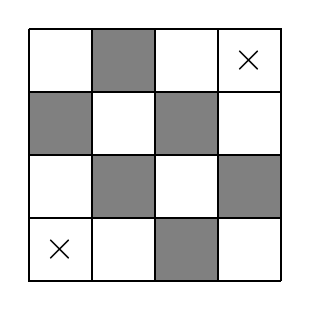
\begin{tikzpicture}[x=0.8cm,y=0.8cm,line width=0.7pt]
    \foreach \p in {(0,0),(2,0),(1,1),(3,1),(0,2),(2,2),(1,3),(3,3)}
        \fill[gray] \p rectangle ++(1,1);
    \draw[step=1] (0,0) grid (4,4);
    \fill[white] (0,0) rectangle (1,1); \draw (0,0) rectangle (1,1);
    \fill[white] (3,3) rectangle (4,4); \draw (3,3) rectangle (4,4);
    \node at (0.5,0.5){\Large \(\times\)};
    \node at (3.5,3.5){\Large \(\times\)};
\end{tikzpicture}}
\end{center}
\end{exemple}

\begin{solution}
Un domino placé sur l'échiquier recouvre deux cases ayant un côté commun,
donc toujours :

\begin{itemize}
    \item une case noire ;
    \item une case blanche.
\end{itemize}

Ainsi \(7\) dominos recouvrent exactement \(7\) cases noires et \(7\) cases
blanches.

Un échiquier \(4\times4\) contient initialement \(8\) cases noires et
\(8\) cases blanches.

Les deux coins opposés retirés ont la même couleur (sur la figure, les cases
noires sont grisées, et les deux coins retirés sont des cases noires). Il reste donc :

\[
6\text{ cases d'une couleur}
\qquad\text{et}\qquad
8\text{ cases de l'autre couleur},
\]

et non \(7\) de chaque couleur.

Ainsi,

\[
\boxed{
\text{L'échiquier mutilé ne peut pas être pavé par des dominos.}
}
\]

On peut le voir comme un invariant : si l'on pose les dominos un par un, la
différence entre le nombre de cases libres d'une couleur et le nombre de cases
libres de l'autre couleur ne change jamais, car chaque domino occupe une case
de chaque couleur. Elle vaut \(8-6=2\) au départ ; elle vaudrait \(0-0=0\) si
tout l'échiquier était pavé.
\end{solution}

\subsection{Sommes et sommes pondérées}\label{sec:sommes-ponderees}

La somme totale des quantités présentes est parfois conservée.

Dans des problèmes plus délicats, la somme ordinaire varie, mais une
\textbf{somme pondérée} reste constante : on multiplie chaque quantité par un
coefficient fixe (son \emph{poids}) avant d'additionner, par exemple
\(x+y+2z\).

\begin{exemple}[trois boîtes]\label{exm:trois-boites}
Trois boîtes \(A\), \(B\) et \(C\) contiennent respectivement \(a\), \(b\) et
\(c\) pierres.

Les opérations autorisées sont les suivantes :

\begin{itemize}
    \item transférer une pierre de \(A\) vers \(B\) ;
    \item retirer deux pierres de \(B\) et placer une pierre dans \(C\).
\end{itemize}

Une opération n'est possible que si la boîte de départ contient assez de
pierres (au moins une dans \(A\), ou au moins deux dans \(B\)).

\begin{center}
\fitfig{%
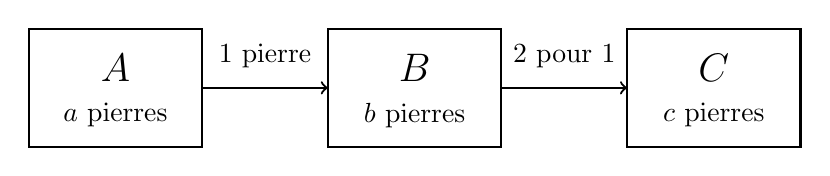
\begin{tikzpicture}[x=1cm,y=1cm,line width=0.8pt]
    \draw (0,0) rectangle (2.2,1.5);
    \draw (3.8,0) rectangle (6,1.5);
    \draw (7.6,0) rectangle (9.8,1.5);
    \node at (1.1,1){\Large \(A\)};
    \node at (1.1,0.4){\(a\) pierres};
    \node at (4.9,1){\Large \(B\)};
    \node at (4.9,0.4){\(b\) pierres};
    \node at (8.7,1){\Large \(C\)};
    \node at (8.7,0.4){\(c\) pierres};
    \draw[->] (2.2,0.75)--(3.8,0.75);
    \draw[->] (6,0.75)--(7.6,0.75);
    \node at (3,1.15){\(1\) pierre};
    \node at (6.8,1.15){\(2\) pour \(1\)};
\end{tikzpicture}}
\end{center}

La somme ordinaire \(a+b+c\) n'est pas conservée par la seconde opération.

Considérons plutôt

\[
I=a+b+2c.
\]

Lors de la première opération,

\[
(a,b,c)\longmapsto(a-1,b+1,c),
\]

donc

\[
I\longmapsto(a-1)+(b+1)+2c=I.
\]

Lors de la seconde opération,

\[
(a,b,c)\longmapsto(a,b-2,c+1),
\]

donc

\[
I\longmapsto a+(b-2)+2(c+1)=I.
\]

Ainsi,

\[
\boxed{I=a+b+2c}
\]

est un invariant.

À partir de l'état

\[
(8,0,0),
\]

on a

\[
I=8.
\]

L'état

\[
(0,1,3)
\]

a pour valeur

\[
I=0+1+2\times3=7.
\]

Il est donc inaccessible.

En revanche,

\[
(0,2,3)
\]

a la même valeur \(I=8\). L'invariant ne suffit pas à conclure : il faut
construire le chemin. On transfère les \(8\) pierres de \(A\) vers \(B\),
puis on applique trois fois la seconde opération :

\[
(8,0,0)\longmapsto\cdots\longmapsto(0,8,0)\longmapsto(0,6,1)
\longmapsto(0,4,2)\longmapsto(0,2,3).
\]

Cet état est donc accessible.
\end{exemple}

\subsection{Le PGCD}\label{sec:pgcd}

\begin{definition}[PGCD]
Le plus grand commun diviseur (PGCD) de deux entiers strictement positifs
\(a\) et \(b\), noté \(\gcd(a,b)\), est le plus grand entier qui divise à la
fois \(a\) et \(b\).
\end{definition}

Il peut également rester constant.

On utilise le fait suivant : si un entier \(d\) divise \(a\) et \(b\), alors
il divise aussi \(a+b\) et \(a-b\).

\begin{proposition}
On en déduit, pour des entiers
strictement positifs \(a\) et \(b\),
\[
\boxed{\begin{gathered}
\gcd(a+b,b)=\gcd(a,b),\\
\text{et, si }a>b,\qquad
\gcd(a-b,b)=\gcd(a,b).
\end{gathered}}
\]
\end{proposition}

\begin{proof}
En effet, un diviseur commun de \(a\) et \(b\) divise \(a+b\) et \(a-b\) ;
réciproquement, un diviseur commun de \(a+b\) et \(b\) divise
\(a=(a+b)-b\), et un diviseur commun de \(a-b\) et \(b\) divise
\(a=(a-b)+b\). Les deux couples ont donc les mêmes diviseurs communs, et en
particulier le même plus grand.
\end{proof}

\begin{exemple}\label{exm:pgcd-couple}
On part d'un couple d'entiers strictement positifs \((a,b)\). Une opération
permet de remplacer l'un des deux nombres par sa somme avec l'autre, ou, si
les deux nombres sont différents, par la différence positive des deux
(le plus grand moins le plus petit).

Les deux nombres restent strictement positifs. Le nouveau nombre est la somme
ou la différence des deux anciens ; inversement, le nombre effacé est la somme
ou la différence des deux nouveaux (par exemple, si l'on remplace \(a<b\) par
\(b-a\), on retrouve \(a=b-(b-a)\)). Le raisonnement ci-dessus montre alors
que l'ancien et le nouveau couple ont les mêmes diviseurs communs : chaque
opération conserve le PGCD.

Ainsi, à partir de

\[
(18,30),
\]

tous les couples accessibles ont pour PGCD

\[
\gcd(18,30)=6.
\]

Il est donc impossible d'atteindre le couple

\[
(17,31),
\]

car

\[
\gcd(17,31)=1\neq 6.
\]
\end{exemple}

\section{Monovariants}\label{sec:monovariants}

Un invariant reste constant. Une autre idée très utile consiste à trouver une
quantité qui varie toujours dans le même sens.

\subsection{Définition}\label{sec:definition-monovariant}

\begin{definition}[Monovariant]
Un \textbf{monovariant} est une quantité \(M\), calculée à partir de l'état,
qui :

\begin{itemize}
    \item soit augmente strictement après chaque opération ;
    \item soit diminue strictement après chaque opération.
\end{itemize}

Autrement dit, si \(S\) est un état et \(S'\) l'état obtenu après une
opération, on a toujours

\[
\boxed{
M(S')>M(S)
}
\]

ou bien toujours

\[
\boxed{
M(S')<M(S).
}
\]
\end{definition}

Supposons que \(M\) prenne des valeurs \textbf{entières}, positives ou nulles,
et diminue strictement à chaque opération. Alors \(M\) diminue d'au moins
\(1\) à chaque opération. Partant de la valeur \(M_0\) de l'état initial, on
ne peut donc pas effectuer plus de \(M_0\) opérations : le processus
s'arrête forcément. De même, un entier qui augmente strictement et ne peut
pas dépasser une valeur fixée ne peut augmenter qu'un nombre fini de fois.

Un monovariant permet notamment de prouver :

\begin{itemize}
    \item qu'un processus doit s'arrêter (avec un monovariant entier comme
    ci-dessus) ;
    \item qu'un état déjà rencontré ne peut jamais réapparaître (il aurait la
    même valeur de \(M\), alors que \(M\) a strictement varié) : le processus
    ne peut donc pas tourner en rond.
\end{itemize}

\subsection{Exemple : l'algorithme des différences}\label{sec:algorithme-differences}

On considère deux entiers strictement positifs \(a\) et \(b\).

Tant qu'ils sont différents, on remplace le plus grand par la différence des
deux nombres (le plus grand moins le plus petit). Les deux nombres restent
strictement positifs.

Par exemple,

\[
(18,30)
\longmapsto
(18,12)
\longmapsto
(6,12)
\longmapsto
(6,6).
\]

La somme

\[
M=a+b
\]

diminue strictement à chaque opération : si \(a>b\), on passe de \(a+b\) à
\((a-b)+b=a\), donc \(M\) diminue de \(b\), qui vaut au moins \(1\).

Elle reste pourtant un entier strictement positif. Elle ne peut donc pas
diminuer indéfiniment.

Le processus doit s'arrêter.

Par ailleurs, cette opération est un cas particulier de celles de l'exemple
précédent, donc le PGCD de \(a\) et \(b\) est invariant. Le processus ne
s'arrête que lorsque les deux nombres sont égaux, à une valeur commune \(d\).
Comme \(\gcd(d,d)=d\), cette valeur commune est le PGCD initial.

Dans l'exemple,

\[
\gcd(18,30)=6.
\]

On obtient bien le couple final

\[
(6,6).
\]

Cet exemple utilise simultanément :

\[
\boxed{\text{un invariant : le PGCD}}
\]

et

\[
\boxed{\text{un monovariant : la somme \(a+b\)}}.
\]

\section{À retenir}\label{sec:retenir}

\begin{retenir}
\begin{itemize}
    \item \textbf{Invariant.} C'est une quantité qui garde la même valeur après
    chaque opération. Si elle n'a pas la même valeur dans l'état initial et
    dans l'état visé, l'état visé est impossible à atteindre.

    \item \textbf{La réciproque est fausse en général.} Deux états qui ont la
    même valeur de l'invariant ne sont pas forcément reliés. Pour prouver
    qu'un état est accessible, on construit une suite d'opérations qui y mène.

    \item \textbf{Monovariant.} C'est une quantité qui augmente strictement à
    chaque opération, ou qui diminue strictement à chaque opération. Un
    entier positif ou nul qui diminue strictement à chaque opération prouve que
    le processus s'arrête.

    \item \textbf{Parité.} Penser à la parité quand chaque opération change une
    quantité d'un nombre pair (par exemple, quand on retourne deux jetons à la
    fois : le nombre de jetons noirs varie de \(-2\), \(0\) ou \(+2\)).

    \item \textbf{Reste modulo \(m\).} Si chaque opération ajoute ou retranche
    un multiple de \(m\), le reste modulo \(m\) ne change pas.

    \item \textbf{Coloriage.} Pour un pavage ou des déplacements sur une
    grille, colorier les cases de sorte que chaque pièce (ou chaque
    déplacement) agisse de la même façon sur chaque couleur, puis compter les
    cases de chaque couleur.

    \item \textbf{Somme pondérée.} Quand la somme ordinaire varie, chercher des
    poids \(w_1,\dots,w_n\) tels que \(w_1x_1+\cdots+w_nx_n\) ne change pas :
    ce que l'opération enlève d'un côté est compensé de l'autre.

    \item \textbf{PGCD.} Quand on remplace un nombre par sa somme ou sa
    différence avec un autre nombre présent, les diviseurs communs, donc le
    PGCD, ne changent pas.
\end{itemize}

\[
\boxed{
\text{Invariant différent}
\Longrightarrow
\text{état inaccessible}
}
\]

\[
\boxed{\begin{gathered}
\text{Entier qui diminue strictement et reste positif}\\
\Longrightarrow\;
\text{le processus finit par s'arrêter}
\end{gathered}}
\]
\end{retenir}

\section{Exercices}\label{sec:exercices}

\subsection*{Exercices de compréhension}

\exochap{recueil-7-01-vingt-jetons}{Vingt jetons}
\exochap{recueil-7-02-ajouter-retrancher}{Ajouter 10 ou retrancher 15}
\exochap{recueil-7-03-cavalier}{Le cavalier}
\exochap{recueil-7-04-invariant-ou-monovariant}{Invariant ou monovariant ?}

\subsection*{Exercices faciles}

\exochap{recueil-7-05-dix-entiers}{Dix entiers et une parité}
\exochap{recueil-7-06-echiquier-6x6}{Échiquier $6\times6$ mutilé}
\exochap{recueil-7-07-couple-84-30}{Le couple $(84, 30)$}
\exochap{recueil-7-08-sommets-triangle}{Nombres aux sommets d'un triangle}

\subsection*{Exercices \texorpdfstring{$+$}{+}}

\exochap{recueil-7-09-trois-boites}{Les trois boîtes}
\exochap{recueil-7-10-pavage-carres}{Pavage par carrés $2\times2$}
\exochap{recueil-7-11-pierres-cercle}{Pierres disposées en cercle}
\exochap{recueil-7-12-produit-invariant}{Produit invariant}

\subsection*{Exercices \texorpdfstring{$++$}{++}}

\exochap{recueil-7-13-jetons-alignes}{Jetons alignés}
\exochap{recueil-7-14-quatre-coins}{Les quatre coins d'un rectangle}
\exochap{recueil-7-15-invariant-monovariant}{Invariant et monovariant}

\section{Problèmes}\label{sec:problemes}

\probleme{recueil-7-pc1-taquin}{Le taquin de quinze pièces}
\probleme{recueil-7-p2-operation-algebrique}{Une opération algébrique}
\probleme{recueil-7-pc3-barres-longueur-3}{Pavage par barres de longueur $3$}
\probleme{recueil-7-pc4-cycle-pair}{Égalisation sur un cycle pair}
\probleme{recueil-7-pc5-suite-transformations}{Une suite de transformations}

% Aucune solution.tex pour ce chapitre : pas de section « Solutions ».
% Quand elles existeront : \ifsolutions\clearpage\section{Solutions}\label{sec:solutions} puis un \solutionde par exercice\fi

\end{document}
